\chapter{Specifikace informačního systému}

S využitím výše uvedené analýzy způsobů správy semestrálních projektů a seznamů pozitivních a negativních prvků je potřeba navrhnout informační systém, jenž by se mohl stát potenciální náhradou větší části služeb. 

Pokud zobecníme správu jednoho projektu a vizualizujeme jeho životní
cyklus~\ref{pic:dia-seq-study-project-lifecycle}, tak to bude především komunikace dvou subjektů -- vyučujícího a studenta\footnote{V grafu \ref{pic:dia-seq-study-project-lifecycle} jsou označené jako \texttt{initiator} a \texttt{executor}.}~--, jež postupně tvoří obsah projektu.

Vyučující zakládá a přiřazuje nebo nabízí projekt studentům na fakultě. Průběh projektu je strukturovaný do jedné, či více iterací, přičemž obsahuje sadu úkolů, které je potřeba splnit. Úkoly zpravidla patří pod určité iterace, aby se jednoznačně definovala zadaná práce. Po vytvoření projektu je o tom student informován a začíná vypracovávat jednotlivé úkoly a tím tvořit obsah projektu. V situaci, kdy je současná iterace splněna, student ji může odevzdat ke kontrole vedoucímu projektu, jenž na základě hotové práce přiděluje určitý počet bodů. Daný postup tvoření a hodnocení obsahu se opakuje do doby, než jsou všechny iterace vyčerpány. V tuto chvíli se projekt považuje za dokončený a vedoucí ho archivuje.


\begin{fig:illustration}
   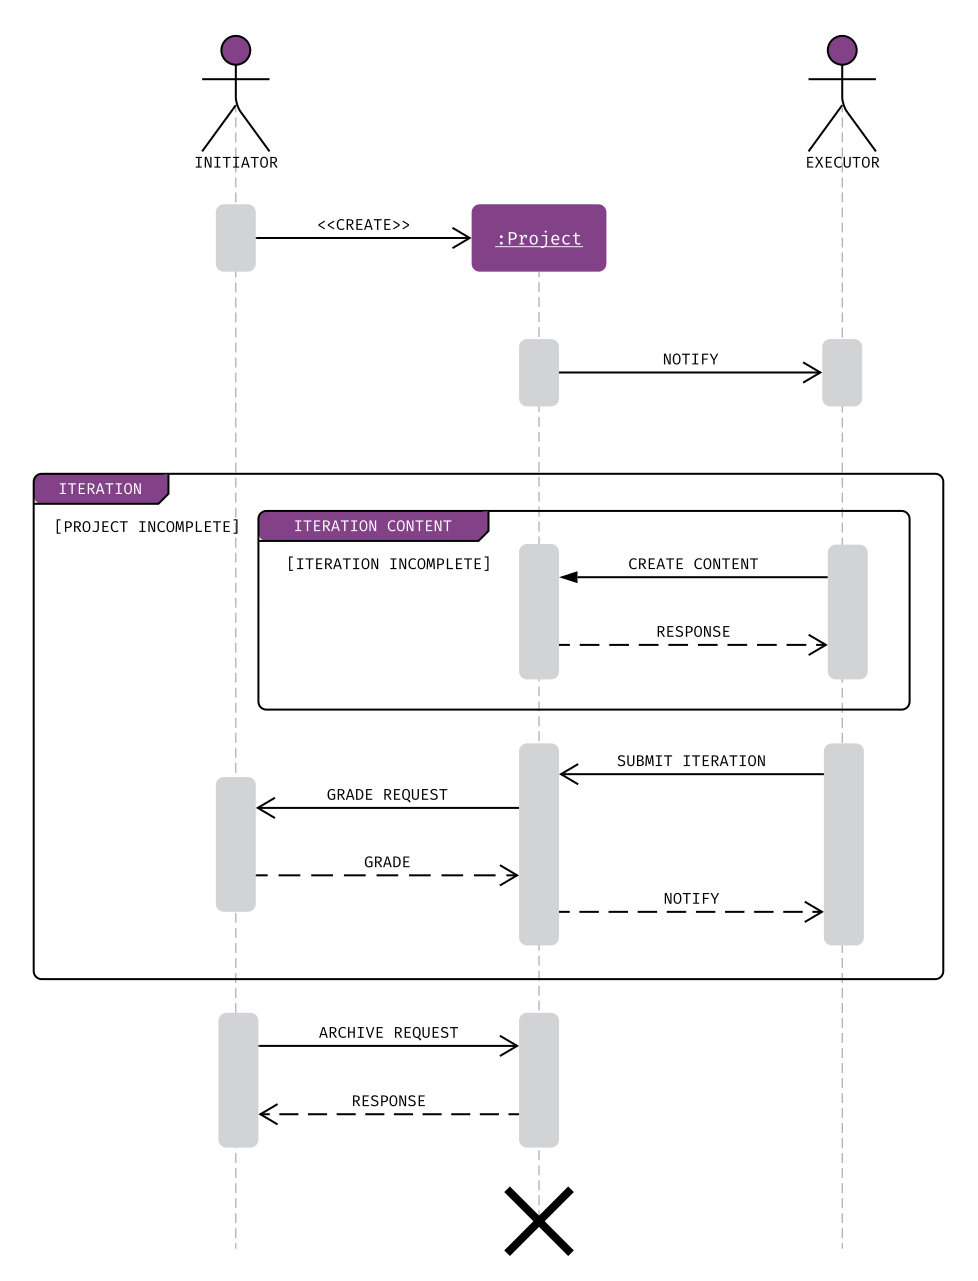
\includegraphics[width=1\textwidth]{images/dia-seq-study-project-lifecycle.pdf}
   \caption[Zobecněný životní cyklus projektu]{Sekvenční diagram zobecněného životního cyklu projektu na \gls{fit} \gls{čvut}}\label{pic:dia-seq-study-project-lifecycle}
\end{fig:illustration}


Podobného způsobu správy se má držet i budoucí \gls{is}, nebude však omezován pouze na vedoucí z řad vyučujících. Projekty bude možné zakládat a řídit běžným studentům, tím bude do jisté míry podporována jejich samostatná činnost.


\section{Požadavky na systém}

Pro definování rozsahu práce slouží funkční a obecné požadavky. Funkční požadavky zachycují jednotlivé funkcionality vytvářené aplikace, jejich logickou stránku a chování. Obecné požadavky, neboli nefunkční, jsou požadavky, jež na systém kladou jistá omezení a tím upřesňují rozsah práce, avšak nedefinují žádnou aktivní složku (například uživatelská funkcionalita nebo serverová činnost). 


\subsection{Funkční požadavky}

\begin{dl}
   \item[FR00 Identita uživatelů]
   Součástí aplikace je uživatelský systém vyjma autorizačního serveru. Aplikace využívá pouze autorizační servery třetích stran, s jejich pomocí probíhá registrace i přihlášení. Identitu uživatele musí být možné přesně určit na všech webových stránkách, kromě skupiny stránek sloužící pro autentizaci či informování o základních náležitostech (například podmínky užití).

   \item[FR01 Globální role]
   Vsechny účastníci \gls{is} mají přidělenou jednu globální roli, která určuje jejich oprávnění v rámci aplikace. Ihned po registraci dostávají výchozí roli standardního uživatele. Existuje speciální role administrátor, jenž má neomezený přístup. Další role představují jiné množiny oprávnění, které jsou definovány v případech užití. U jednotlivých globálních rolí lze nastavit kritérium důvěryhodnosti. Uživatelé s danou rolí jsou v \gls{is} uvedeny se speciálním označením vedle uživatelského jména. Aplikace umožňuje měnit roli uživatele, přidávat nové role a měnit oprávnění.

   \item[FR02 Osobní informace uživatelů]
   Aplikace umožňuje účastníkům \gls{is} prohlížet si svoje osobní informace, které jsou uchovávány na serveru. Existuje funkcionalita pro odstranění bez možnosti obnovení (v případě nutnosti zachování určitých činností budou dané činnosti zanonymizovány).

   \item[FR03 Upozornění]
   Aplikace posílá účastníkům \gls{is} upozornění po každé významné činnosti (například ohodnocení práce, archivace projektu\dots{}), jež se jich přímo týká. Upozornění existují pouze v rámci \gls{is} a představují jednoduchou textovou zprávu. Účastníci mají možnost zobrazit svoje upozornění a označit je jako přečtené/nepřečtené nebo úplně odstranit.

   \item[FR04 Projekt -- Životní cyklus]
   Aplikace umožňuje účastníkům \gls{is} zakládat vlastní projekty, ve kterých se automaticky stávají vedoucími. Po založení je možné vytvořit tým, definovat cíle a začít tvořit obsah. V případě neaktuálnosti projektu se dá odstranit, tím zcela zanikne, nebo archivovat, pak existuje možnost ho kdykoliv obnovit. Archivací se zakáže veškerá činnost uživatelů na~daném projektu kromě rušení archivace a odchodu uživatelů z projektového týmu.

   \item[FR05 Projekt -- Správa dat]
   Každý projekt je definován množinou dat, jež ho popisují a prezentují. Data se dělí na vždy veřejné, skryté a volitelně skryté. Mezi veřejné patří: 

   \begin{ulnar}
      \item kategorie,
      \item název,
      \item datum založení,
      \item veřejný popis,
      \item seznam členů projektového týmu,
      \item tagy,
      \item status archivace.
   \end{ulnar}


   Skryté (dostupné pouze pro členy) jsou: 

   \begin{ulnar}
      \item seznam iterací a úkolů, 
      \item interní popis projektu, 
      \item snapshoty iterací a jejich hodnocení.
   \end{ulnar}
   

   Za volitelně skryté se považují vakantní pozice a samotný obsah.

   \item[FR06 Projekt -- Kategorie a tagy]
   Aplikace umožňuje třídění projektů do jednotlivých skupin s pomocí kategorií a tagů. Každý založený projekt povinně patří právě do jedné kategorie, která určuje jeho primární zaměření. Kategorie lze zakládat, upravovat a odstraňovat, pokud jsou prázdné. V případě nutnosti přesnější specifikace projektu je možné použít tagy, které budou primárně sloužit jako prostředek pro vyhledávání.

   \item[FR07 Projekt -- Tým a role]
   Na tvorbě obsahu projektu se podílí uživatelé s příslušným oprávněním. Pro přiřazování oprávnění slouží projektové role. Dle logického hlediska se dají rozdělit pouze na tři typy -- vedoucí, spolupracovník a návštěvník.

   \newpage
   Vedoucí mají neomezený přístup z hlediska práv. Prvním vedoucím projektu se vždy stává uživatel, jenž daný projekt založil. Každý vedoucí může prohlásit jiného člena týmu za vedoucího. Odejít z této role však lze pouze v případě, že~v projektu zůstane alespoň jeden vedoucí.

   Pravým opakem vedoucích jsou návštěvníci, kteří mají právo pouze prohlížet obsah, nikoliv do něj zasahovat. Volné přihlašování na roli návštěvníka lze zakázat, či povolit.

   Speciálním typem role je spolupracovník, který slouží pouze jako nadskupina pro množinu kapacitně omezených pracovních míst. Pracovní místa jsou definovány vedoucím pro inzerci náboru členů týmu. V případě, že je otevřené přihlašování, běžní uživatelé se mohou dobrovolně hlásit na vakantní pozice. Pokud vedoucí má status důvěryhodného uživatele, tak může přidat člena týmu i bez jeho souhlasu.

   \item[FR08 Projekt -- Vyhledávání]
   Aplikace umožňuje uživatelům vyhledávat existující projekty podle zadaných kritérií, pokud vedoucí projektu povolil jeho vyhledávání. Mezi filtry pro vyhledávání patří: 

   \begin{ulnar}
      \item stav archivace, 
      \item projekty, ve kterých je aktuální uživatel vedoucím, 
      \item projekty, do kterých má aktuální uživatel přístup, 
      \item dle kategorie, 
      \item dle tagů.
   \end{ulnar}
   

   \item[FR09 Projekt -- Iterace a úkoly]
   Aplikace umožňuje definovat plánovaný průběh projektu v podobě iterací a úkolů. Iterace je dlouhodobá, má název a plánované datum dokončení, slouží jako nadskupina pro jednotlivé úkoly. Úkoly se skládají z názvu, popisu, maximálního a minimálního počtu bodů. V průběhu tvoření obsahu projektu jednotlivé části obsahu označují úkoly jako splněné.

   \item[FR10 Projekt -- Správa obsahu]
   Aplikace umožňuje vedoucím a spolupracovníkům projektu tvořit jeho obsah. Ten může být soukromý, neboli dostupný pouze pro členy projektu, nebo veřejný, v tomto případě je dostupný pro všechny účastníky \gls{is}.

   Obsah je členěn do částí. Každá část tvoří samostatný celek, jenž se zakládá na určité šabloně (například šablona pro text, obrázek, graf), a může označovat jeden či několik úkolů za splněné. Seřazené části dávají výsledný obsah projektu, jenž se dá prohlížet online, případně zobrazit upravený pro tisk.

   \item[FR11 Projekt -- Snímky iterací]
   Aplikace poskytuje funkcionalitu vytvoření snímku určité iterace. Je to záznam aktuálního stavu všech částí obsahu, které splňují alespoň jeden z úkolů vybrané iterace. Tento záznam je dostupný pouze pro~čtení a existuje nezávisle na obsahu projektu. Snímek lze po vytvoření odevzdat pro ohodnocení, které spočívá v přiřazování bodů s volitelným komentářem k jednotlivým úkolům snímku. Dané hodnocení snímku se promítá do celkového přehledu iterací projektu. V případě, že existuje víc ohodnocených snímků jedné iterace, tak se bere nejnovější (nejpozději upravené). Existuje možnost změnit ohodnocení snímku, ale danou činnost může provádět pouze uživatel, jenž je původním hodnotitelem snímku.

   \item[FR12 Projekt -- Důvěryhodnost]
   Aplikace označuje projekt za důvěryhodný, pokud alespoň jeden z vedoucích je důvěryhodný. To se projevuje v podobě speciálního značení vedle názvu projektu.

   \item[FR13 Omezení obsahu \gls{is} pouze na projekty]
   Informační systém je pouze služba pro správu prací, nebude poskytovat žádnou jinou funkcionalitu pro uchovávaní dat s rychle stárnoucí hodnotou. Tím se zamezí nutnost neustálého udržování aplikace z hlediska obsahu.

\end{dl}


\subsection{Obecné požadavky}

\begin{dl}
   \item[NR00 Veřejné API]
   Aplikace nabízí otevřené \gls{api} pro vývojáře klientských aplikací.

   \item[NR01 Dokumentace]
   Součástí aplikace je vývojářská a uživatelská dokumentace.

   \item[NR02 Rozšiřitelnost]
   Aplikace bere v ohled budoucí rozvoj aplikace a zvyšující se nároky na server.

   \item[NR03 Optimalizace uživatelského rozhraní]
   Webové rozhraní aplikace je adaptované pro základní prohlížeče (Google Chrome, Mozilla Firefox, Apple Safari) a je responzivního nebo adaptivního typu optimalizované pro dvě velikosti obrazovek -- mobilních telefonů (pod 1~000~px) a desktopových počítačů (nad 1~000~px).

   \newpage
   \item[NR04 GDPR] 
   Aplikace splňuje požadavky \gls{gdpr}.

   \item[NR05 Jazykové verze] 
   Rozhraní aplikace bude dostupné v anglickém jazyce.
\end{dl}

\section{Uživatelské činnosti}

\subsection{Uživatelské role}

Z funkčních požadavků plyne, že každý uživatel v systému má vždy přiřazenou právě jednu z globálních rolí. Tím se stanovují jejich práva na provádění určitých činností v rámci \gls{is}.

Základní množinu uživatelských rolí tvoří \texttt{administrator}, \texttt{banned}, \texttt{user}, \texttt{authority} a imaginární role \texttt{guest}, jenž se přímo nevyskytuje v \gls{is} a pouze označuje neautorizované osoby. Diagram \ref{pic:dia-actors-global} znázorňuje logickou dědičnost těchto rolí na základě přístupových práv. Administrátor (\texttt{administrator}) systému má povolené všechny typy činností, zablokovanému (\texttt{banned}) uživateli je povoleno pouze přihlášení a přehled soukromých dat. Přístupová práva ostatních rolí jsou smíšená a jsou podrobně definována v seznamu případů užití.


\begin{fig:illustration}
   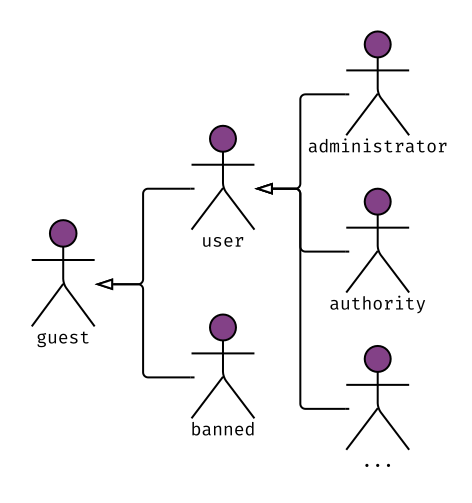
\includegraphics[width=0.5\textwidth]{images/dia-actors-global.pdf}
   \caption{Diagram logické dědičnosti globálních uživatelských rolí v systému}\label{pic:dia-actors-global}
\end{fig:illustration}


V každém projektu uživatelé budou nabývat sekundárních rolí, jež budou mít vliv pouze na daný projekt. Mezi ně patří vedoucí projektu (\texttt{leader}), skupina uživatelsky definovaných rolí spolupracovníků (\texttt{contributor}) a návštěvníci (\texttt{visitor}) s právy pouze pro čtení. Jejich logická dědičnost je znázorněna v diagramu \ref{pic:dia-actors-project}.


\begin{fig:illustration}
   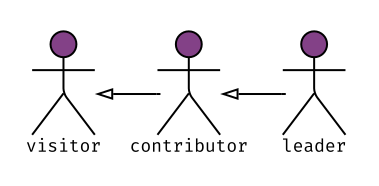
\includegraphics[width=0.5\textwidth]{images/dia-actors-project.pdf}
   \caption{Diagram logické dědičnosti uživatelských rolí v projektu}\label{pic:dia-actors-project}
\end{fig:illustration}



\subsection{Případy užití}

Případ užití neboli \gls{uc} je činnost, k vykonávání které dochází ze strany uživatele \gls{is} (buď člověka nebo jiného systému). Jednotlivé činnosti jsou řazeny do~dříve definovaných funkčních požadavků a během implementování jsou přímo promítány na jednotlivé typy oprávnění, jež budou přiřazovány globálním a projektovým rolím.


\begin{dlnar}
   \item[FR00] \textbf{Identita uživatelů}

   \begin{dlnar}
      \item[UC00]
      \texttt{guest} se může zaregistrovat nebo přihlásit do \gls{is} jedním z dostupných serverů třetích stran.
   \end{dlnar}
\end{dlnar}



\begin{dlnar}
   \item[FR02] \textbf{Globální role}

   \begin{dlnar}
      \item[UC01] 
      \texttt{administrator} může měnit roli uživatele. 

      \item[UC02] 
      \texttt{administrator} může přidávat nové role a upravovat oprávnění. 

      \item[UC03]
      \texttt{administrator} může upravovat oprávnění jednotlivých rolí.

      \item[UC04] 
      \texttt{administrator} může upravovat důvěryhodnost jednotlivých rolí.
   \end{dlnar}
\end{dlnar}


\begin{dlnar}
   \item[FR03] \textbf{Osobní informace uživatelů}
 
   \begin{dlnar}
      \item[UC05] 
      Jakýkoliv účastník \gls{is} může prohlédnout svoje osobní informace. 

      \item[UC06] 
      Jakýkoliv účastník \gls{is} může odstranit svůj účet.
   \end{dlnar}
\end{dlnar}


\begin{dlnar}
   \item[FR04] \textbf{Upozornění}
 
   \begin{dlnar}
      \item[UC07] 
      \texttt{user} může zobrazit, upravit stav nebo odstranit svoje upozornění.
   \end{dlnar}
\end{dlnar}


\begin{dlnar}
   \item[FR05] \textbf{Projekt -- Životní cyklus}
   
   \begin{dlnar}
      \item[UC08]
      \texttt{user} může založit projekt. 

      \item[UC09]
      \texttt{user} s projektovou rolí \texttt{leader} může odstranit projekt. 

      \item[UC10]
      \texttt{user} s projektovou rolí \texttt{leader} může nastavit stav archivace.
   \end{dlnar}
\end{dlnar}


\begin{dlnar}
   \item[FR06] \textbf{Projekt -- Správa dat}
   
   \begin{dlnar}
      \item[UC11]
      \texttt{user} s projektovou rolí \texttt{leader} může upravit veřejné informace a interní popis projektu.
   \end{dlnar}
\end{dlnar}


\begin{dlnar}
   \item[FR07] \textbf{Projekt -- Kategorie a tagy}
 
   \begin{dlnar}
      \item[UC12]
      \texttt{user} s projektovou rolí \texttt{leader} může přidávat, upravovat a odstranovat tagy projektu. 

      \item[UC13]
      \texttt{authority} může zakládat kategorie. 

      \item[UC14]
      \texttt{authority} může upravovat kategorie. 

      \item[UC15]
      \texttt{administrator} může odstraňovat kategorie, pokud neobsahuje ani jeden projekt.
   \end{dlnar}
\end{dlnar}


\begin{dlnar}
   \item[FR08] \textbf{Projekt -- Tým a role}
 
   \begin{dlnar}

      \item[UC16] 
      \texttt{user} s projektovou rolí \texttt{leader} může přidávat, upravovat a odstraňovat projektové role typu \texttt{contributor}.

      \item[UC17]
      \texttt{authority} s projektovou rolí \texttt{leader} může přidávat uživatelé do týmu.

      \item[UC18] 
      \texttt{user} s projektovou rolí \texttt{leader} může měnit projektovou roli uživatele.

      \item[UC19]
      \texttt{user} s projektovou rolí \texttt{leader} může odstraňovat uživatelé z týmu.

      \item[UC20] 
      \texttt{user} s projektovou rolí \texttt{leader} může povolovat nebo zakazovat volné přihlášení do projektové role \texttt{visitor}.

      \item[UC21] 
      \texttt{user} s projektovou rolí \texttt{leader} může povolovat nebo zakazovat volné přihlášení do projektových rolí typu \texttt{contributor}.

      \item[UC22]
      \texttt{user} se může hlásit na vakantní místo.
   \end{dlnar}
\end{dlnar}


\begin{dlnar}
   \item[FR09] \textbf{Projekt -- Vyhledávání}
   
   \begin{dlnar}
      \item[UC23] 
      \texttt{user} může vyhledat projekt, pokud je projekt zařazen do seznamu pro vyhledávání.

      \item[UC24]
      \texttt{user} s projektovou rolí \texttt{leader} může přidávat nebo odebírat projekt ze~seznamu pro vyhledávání.
   \end{dlnar}
\end{dlnar}


\begin{dlnar}
   \item[FR10] \textbf{Projekt -- Iterace a úkoly}
   
   \begin{dlnar}
      \item[UC25] 
      \texttt{user} s projektovou rolí \texttt{leader} může přidávat, upravovat a odstraňovat iterace a úkoly.
   \end{dlnar}
\end{dlnar}


\begin{dlnar}
   \item[FR11] \textbf{Projekt -- Správa obsahu}
 
   \begin{dlnar}
      \item[UC26] 
      \texttt{user} s projektovou rolí \texttt{contributor} může zakládat, upravovat a odstraňovat části v obsahu. 

      \item[UC27] 
      \texttt{user} s projektovou rolí \texttt{visitor} může zobrazit obsah.

      \item[UC28] 
      \texttt{user} s projektovou rolí \texttt{visitor} může zobrazit obsah pro tisk.
   \end{dlnar}
\end{dlnar}


\begin{dlnar}
   \item[FR12] \textbf{Projekt -- Snímky iterací}
 
   \begin{dlnar}
      \item[UC29]
      \texttt{user} s projektovou rolí \texttt{contributor} projektu může vytvořit snímek.

      \item[UC30] 
      \texttt{user} s projektovou rolí \texttt{visitor} projektu může zobrazit snímek.

      \item[UC31] 
      \texttt{user} s projektovou rolí \texttt{contributor} projektu může odevzdat snímek.

      \item[UC32]
      \texttt{authority} s projektovou rolí \texttt{leader} může ohodnotit snímek, pokud je odevzdaný.
      
      \item[UC33]
      \texttt{authority} s projektovou rolí \texttt{leader} může změnit hodnocení snímku, pokud je jeho hodnotitelem.

      \item[UC34]
      \texttt{user} s projektovou rolí \texttt{leader} může odstranit snímek, pokud nebyl ohodnocen.  
   \end{dlnar}
\end{dlnar}

\section{Primární aktivity}

Z celé množiny funkcionalit \gls{is} lze vyčlenit několik primárních aktivit, na které budou uživatelé klást největší důraz při práci. Dané činnosti, vzhledem k jejich důležitosti, jsou znázorněny do \gls{uml} diagramů aktivit nebo podrobně zanalyzovány.


% --------------------------------------------------------------------------------------------------
% Autentizace
% --------------------------------------------------------------------------------------------------


\subsection{Autentizace uživatelů}

Základní a prvotní činností \gls{is} je registrace či následné přihlášení neautentizovaných uživatelů. Vzhledem k absenci vlastního autorizačního serveru jsou využívány autorizační servery třetích stran.

Cyklus autentizace přes vybranou službu (viz obrázek~\ref{pic:dia-ak-auth}) začíná uživatelským požadavkem na server. Informační systém přesměruje uživatele na stránky třetí strany, kdy v případě první návštěvy bude uživatel dotázán na povolení poskytovaní jistých osobních informací. V případě odmítnutí je ukončen celý proces autentizace. Pokud uživatel povolil poskytování informací, nebo ho již měl schválený, tak autorizační server posílá potřebná data na server \gls{is}.

Dle poskytnutých informací server ověřuje, zda se jedná o nového uživatele, pak zakládá nový účet se všemi náležitostmi (přiřazení výchozí role, oznámení apod.), nebo o již existujícího, potom kontroluje, zda není potřeba aktualizovat některé informace vzhledem k údajům (údaje, které nemají přímý vliv na identifikaci -- jméno, email apod.).

Po vytvoření, či aktualizaci databáze se vytváří unikátní autorizační klíč, jenž je následně předán klientské aplikaci. Tento klíč je uložen je uložen na klientovi a používán v případě autorizovaných požadavků na server.


\begin{fig:illustration}
   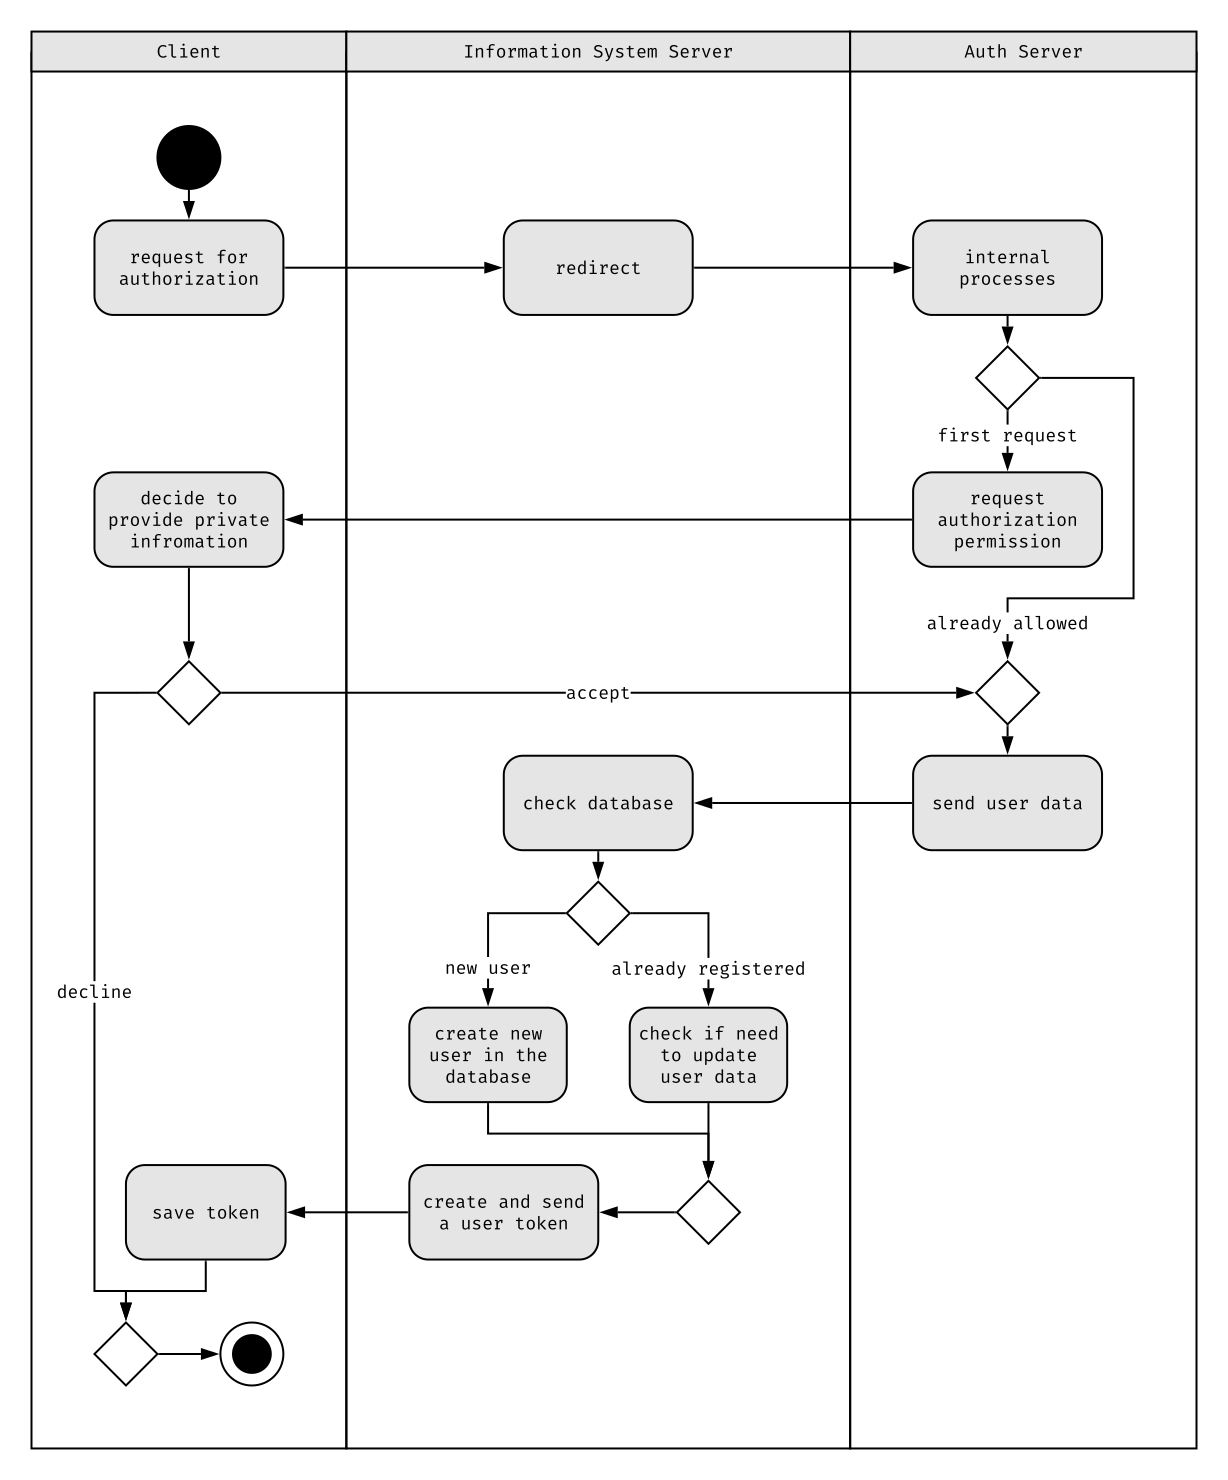
\includegraphics[width=1\textwidth]{images/dia-ak-auth.pdf}
   \caption[Diagram procesu autentizace]{Diagram procesu autentizace}\label{pic:dia-ak-auth}
\end{fig:illustration}


% --------------------------------------------------------------------------------------------------
% Správa projektu
% --------------------------------------------------------------------------------------------------


\subsection{Správa obsahu projektu}

Hlavním cílem projektového týmu bude tvorba obsahu pro plnění úkolů v iteracích. Obsah se skládá z jednotlivých částí, které uchovávají svoje data -- samotný text či jiné informace, název šablony, jenž bude v předem definované podobě zobrazovat informace části uživateli, a seznam úkolů, které tato část splňuje. 

Vznik a správa částí je plně řízena vedoucími a spolupracovníky projektu. Návštěvníci a jiní uživatelé mohou pouze zobrazit obsah (pokud na to mají právo dle globální role a nastavení projektu).

V dané specifikaci všechny části mají být nezávislé, ale pro budoucí rozvoj je třeba počítat se snadno rozšiřitelnou strukturou, aby se dala nastavit výměna dat ve sdíleném úložišti. Celkový průběh generování obsahu popisuje diagram na obrázku~\ref{pic:dia-ak-content} -- po požadavku uživatele zobrazit obsah jsou staženy části projektu do prohlížeče a zanalyzovány. Na~základě analýzy vzniká seznam potřebných šablon, které jsou rovněž staženy ze serveru a následně použity pro generování obsahu z dat každé části. V případě chybějící nebo jinak poškozené šablony či dat části je zobrazena chyba.

\begin{fig:illustration}
   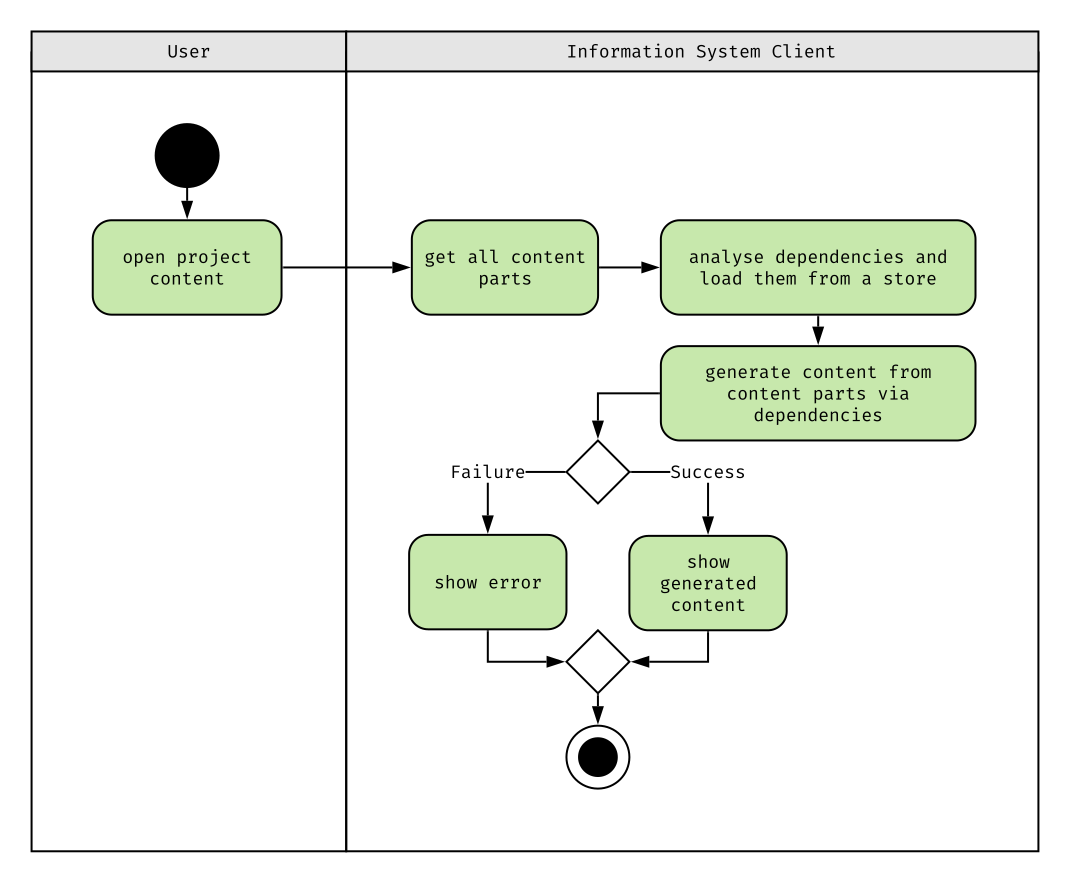
\includegraphics[width=1\textwidth]{images/dia-ak-content.pdf}
   \caption{Diagram generování obsahu projektu}\label{pic:dia-ak-content}
\end{fig:illustration}


% --------------------------------------------------------------------------------------------------
% Vyhledávání projektů
% --------------------------------------------------------------------------------------------------


\subsection{Vyhledávání projektů}

Pro většinu uživatelů bude veškerá činnost v \gls{is} začínat vyhledáváním potřebného projektu. Důvodem může být pokračování v tvorbě obsahu, snaha připojit se k existujícímu týmu, zobrazení existujících dat apod. Z uživatelského hlediska je vhodné mít pro všechny případy vyhledávání dva základní seznamy:

\begin{ulnar}
   \item seznam se všemi veřejně přístupnými projekty
   \item seznam projektů, v nichž je uživatel uveden jako účastník
\end{ulnar}

Seznam přístupných projektů bude určen především pro vyhledávání cizích projektů a dle předpokladu bude méně využívaný, než seznam s uživatelskými projekty. Filtrování obou seznamů bude založeno na volbě obecných vlastností:

\begin{ulnar}
   \item kategorie,
   \item jméno projektu,
   \item stav archivace,
   \item důvěryhodnost (majitel projektu je důvěryhodný),
   \item stav volného přihlašování do projektu,
   \item projekty, do kterých má uživatel přístup,
   \item projekty, ve kterých je uživatel vedoucím.
\end{ulnar}

Následně však může být upřesněno filtrováním dle volitelných štítků. Zavádění podkategorií nebo jiných přesně stanovených seznamů je nevhodné, protože by omezovalo uživatelskou činnost. Štítky představují volnou formu klíčových slov. Jsou ukládány při prvním použití a následně nabízeny všem uživatelům během upravování štítků.


% --------------------------------------------------------------------------------------------------
% Nabídka pozic
% --------------------------------------------------------------------------------------------------



\subsection{Nabídka pozic}

Poslední aktivitou, na kterou bude kladen důraz v \gls{is}, je týmová práce a nabídka vakantních míst. Diagram aktivit na obrázku~\ref{pic:dia-ak-role-assing} zachycuje průběh náboru vývojářského týmu. Nejdřív vedoucí definuje vakantní pozice, které jsou potřeba do projektového týmu a jejich kapacitu (například 5 volných míst pro vývojáře). Po otevření volného přihlašování do~rolí se čeká, až uživatelé najdou projekt, projeví zájem o jednu z daných pozic a odešlou požadavek, že se o danou roli chtějí ucházet. \gls{is} se pokusí začlenit uživatele do~týmu. V případě, že už je součástí projektu, tak pouze změní roli.


\begin{fig:illustration}
   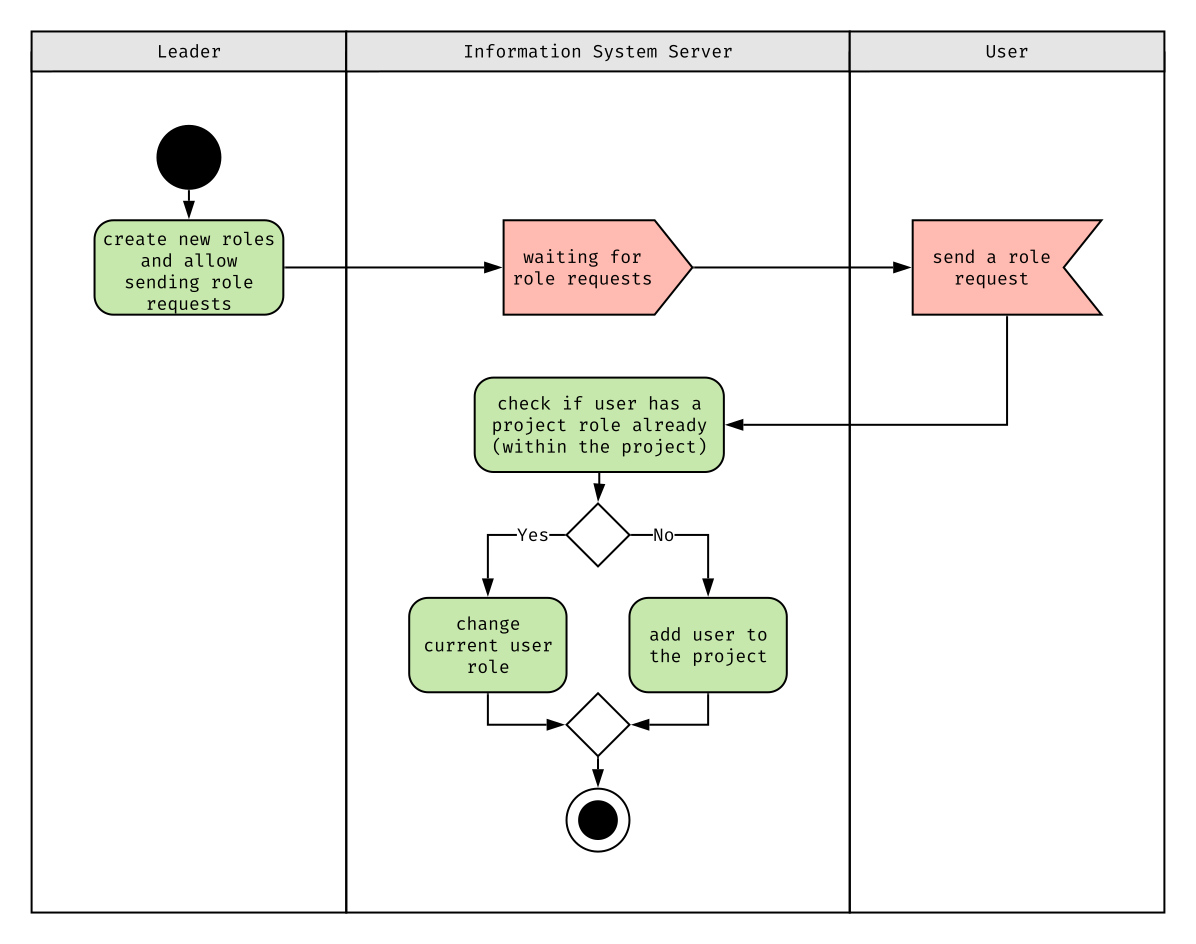
\includegraphics[width=1\textwidth]{images/dia-ak-role-assing.pdf}
   \caption[Diagram průběhu náboru týmu]{Diagram průběhu náboru vývojářského týmu}\label{pic:dia-ak-role-assing}
\end{fig:illustration}

\newpage
Daný proces přiřazování projektové role uživateli mohou ignorovat vedoucí projektů se statusem důvěryhodného účastníka systému. Mají právo přidávat uživatelé do~vlastních projektů bez jejich souhlasu. V tomto případě rovněž neplatí omezení kapacity rolí.
